\begin{figure}[h]
\uwsinglespace
\begin{center}
\begin{minipage}{0.9\textwidth}
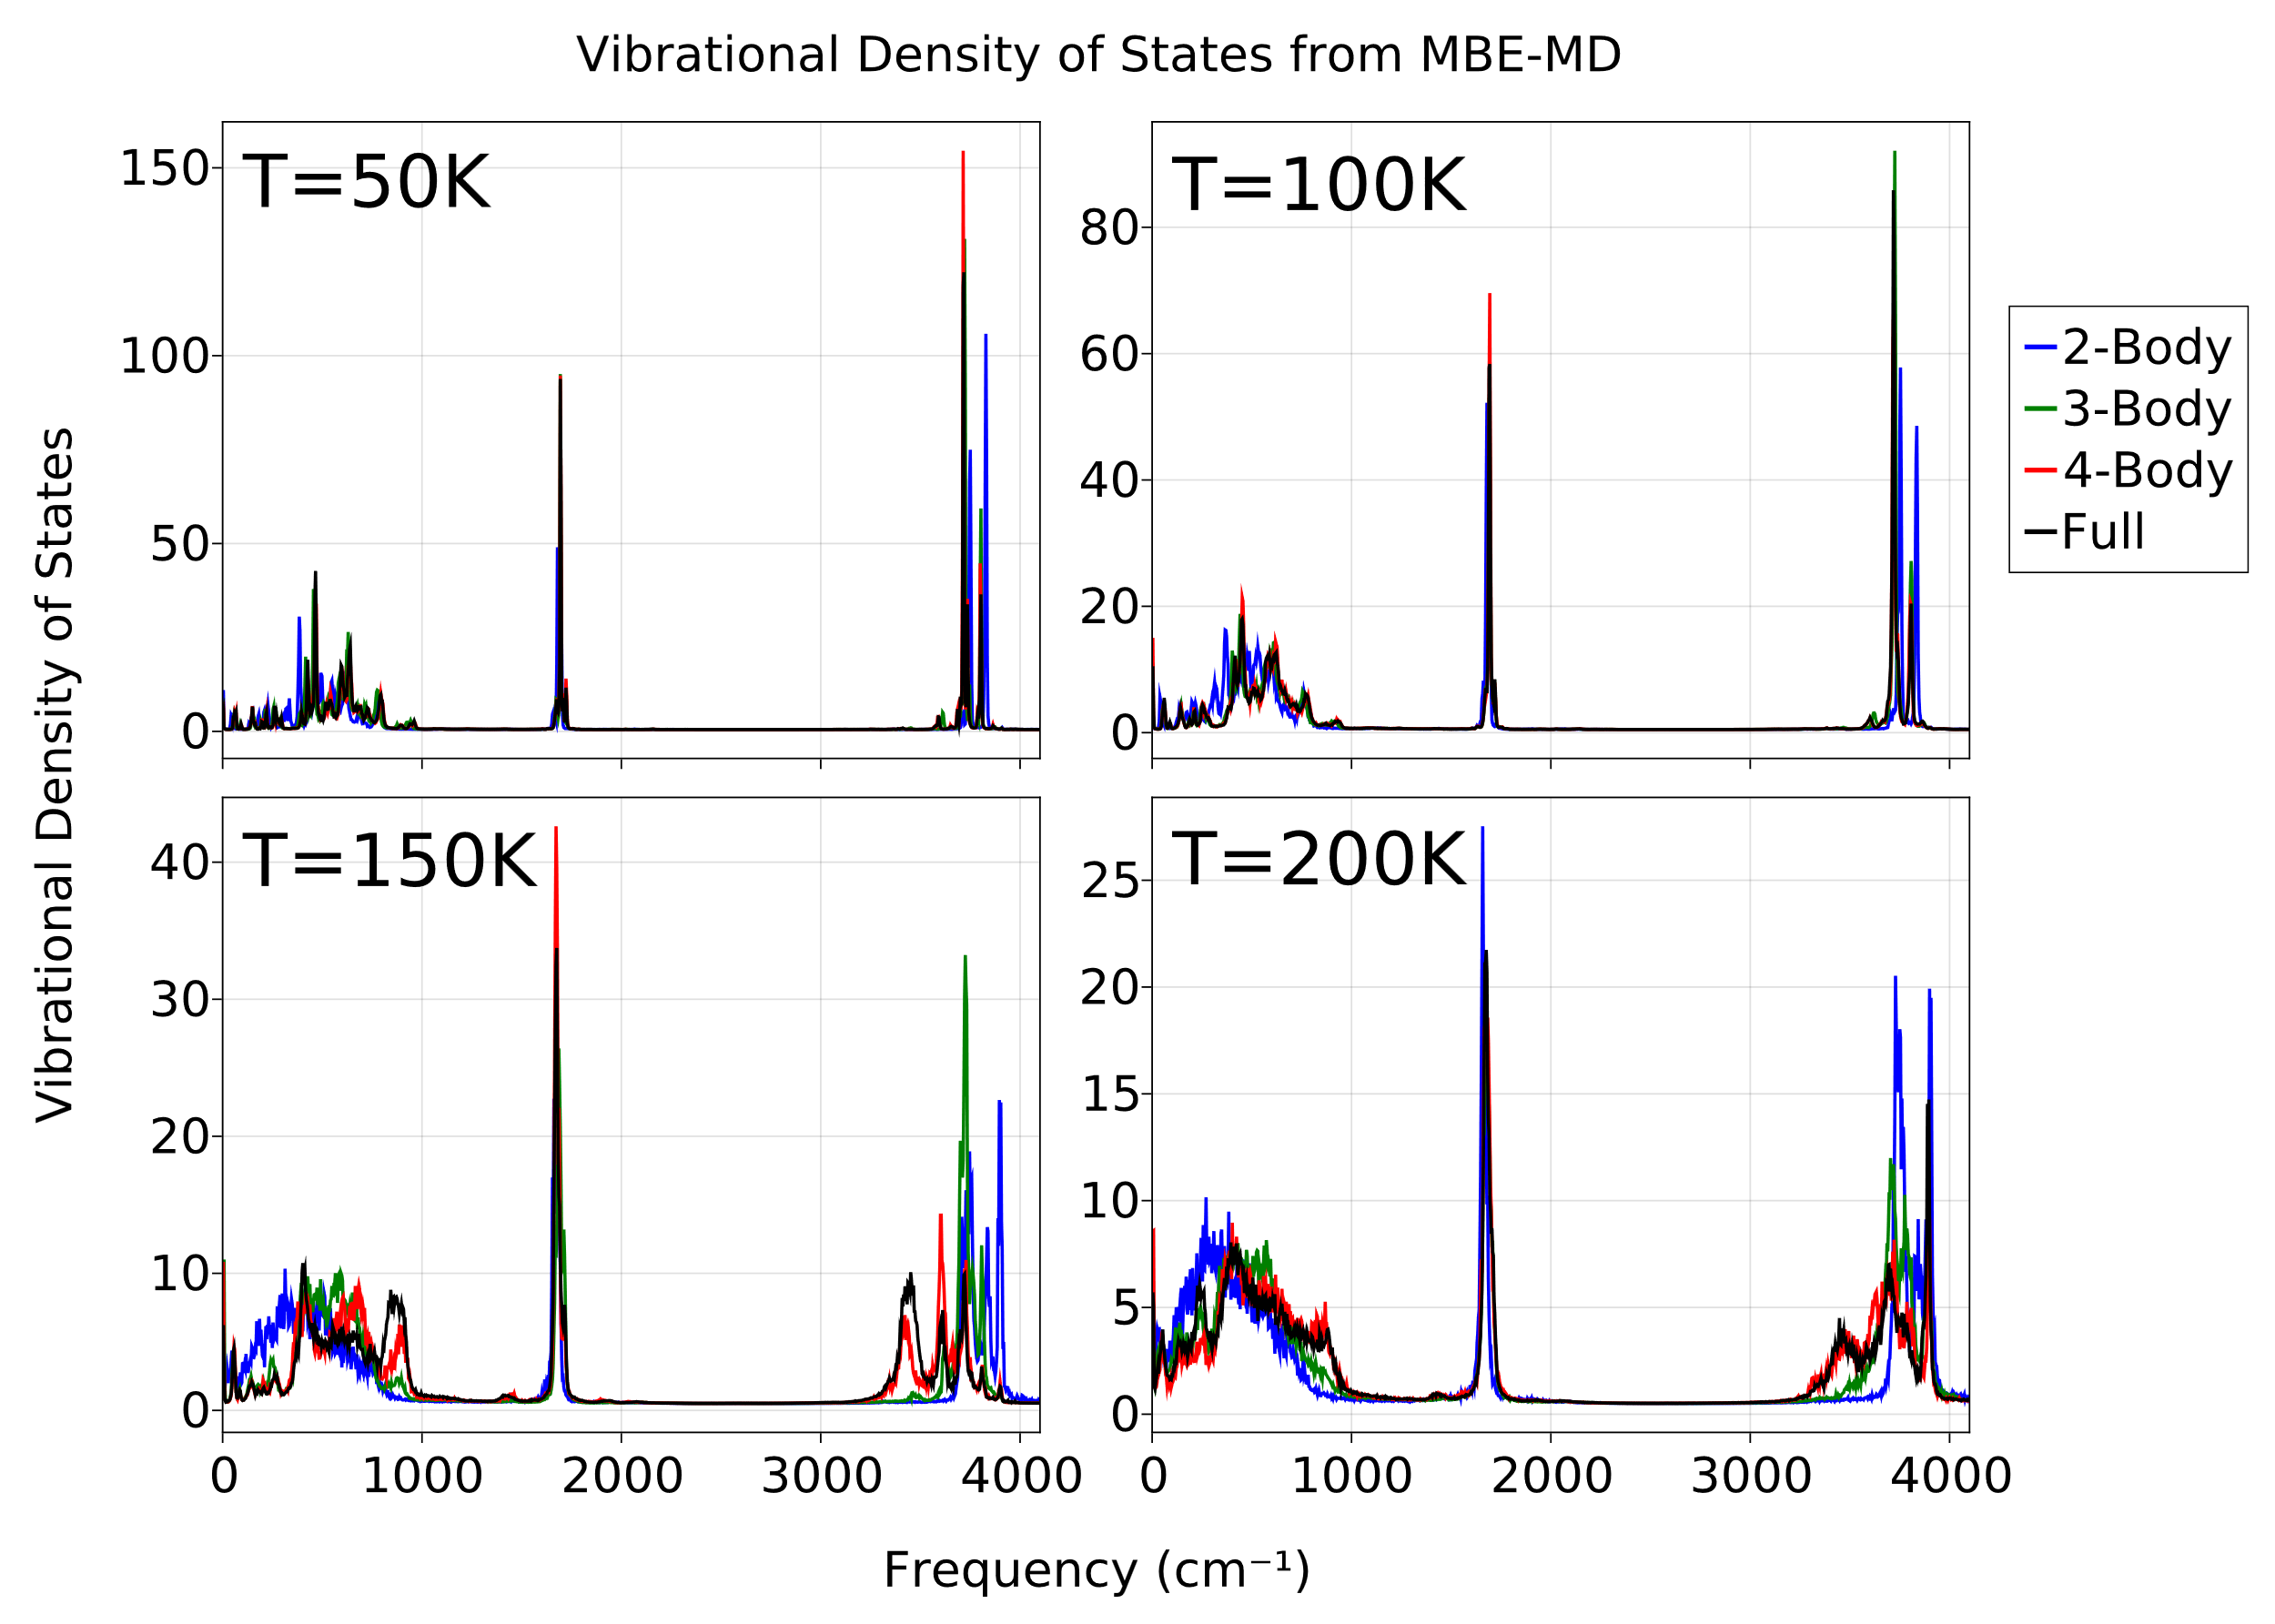
\includegraphics[width=\textwidth]{Figures/Chapter_4/ch4_figure_4.png}
\end{minipage}
\end{center}
\caption[Vibrational density of states as calculated from a 2-, 3-, and 4-body representation of the forces at temperatures of 50K, 100K, 150K, and 200K. The VDOS calculated from the full system is also shown for comparison. Note that each panel has a different y-axis because thermal broadening results in significantly decreased maximum intensity.]{Vibrational density of states as calculated from a 2-, 3-, and 4-body representation of the forces at temperatures of 50K, 100K, 150K, and 200K. The VDOS calculated from the full system is also shown for comparison. Note that each panel has a different y-axis because thermal broadening results in significantly decreased maximum intensity.}
\label{fig:MBE_MD_F4}
\end{figure}